\documentclass[crop=false, class=book]{standalone}

\usepackage{graphicx}
\usepackage[italian]{varioref}
\usepackage{copyrightbox}
\usepackage{subfig}

\begin{document}
		
	\chapter{Anchor and Trackable}
	\label{cap:anchor}
	
		ARCore definisce gli Anchor per assicurare che gli oggetti virtuali rimangano nella stessa posizione e vengano tracciati nel tempo. L'ambiente circostante può cambiare, ed è necessario che la posizione di questi oggetti
		rimanga stabile \cite{gumgumcu2019arcore}. Gli Anchor sono disposti in insieme di punti o piani rappresentati da oggetti di tipo \verb|Trackable|.\\
		Gli oggetti \verb|Trackable| rappresentano la forma geometrica sulla quale verranno definiti gli anchor.
		Su questi oggetti possono essere invocati 3 metodi:
		\begin{itemize}
			\item \verb|createAnchor(pose: Pose)| crea un anchor in una posa che è definita nel \verb|Trackable| corrente. Il tipo di oggetto \verb|Trackable| definirà il modo con cui l'anchor verrà disposto e la modalità di aggiornamento della sua posa mentre il modello del mondo varia.
			\item \verb|getAnchors()| restituisce tutti gli anchor presenti nel dato \verb|Trackable|.
			\item \verb|getTrackingState()| restituisce un oggetto \verb|TrackingState| che rappresenta lo stato del \verb|Trackable|. Questo stato può essere: \verb|PAUSED| quando il rilevamento viene perso ma potrebbe riprendere in futuro; \verb|STOPPED| quando viene fermato e non verrà più ripreso; \verb|TRACKING| se viene tracciato il determinato \verb|Trackable|.
		\end{itemize}
	
		\noindent
		La definizione di anchor e lo stato di tracciamento sono stati molto importanti per la definizione delle funzionalità principali della nostra applicazione.\\
	 	In base alla modalità l'applicazione offre funzionalità differenti:
		
	 	\begin{itemize}
	 		\item \emph{Plane Detection}: ARCore rileva dei piani (\verb|Trackable|) sui quali è possibile posizionare degli animali virtuali. In particolare, quando l'utente tocca un punto preciso del piano viene definito un anchor sul quale verrà renderizzato il modello 3d dell'animale. Si veda il listing~\vref{lst: Definizione Anchor in Plane Detection}.
	 	
	 		\item \emph{Augmented Images}: in ciascun frame viene controllato se lo stato di un'immagine aumentata è \verb|TRACKING|; in questo caso l'immagine viene riconosciuta e viene definito un anchor nel suo centro nel quale verrà renderizzato il modello del pianeta corrispondente. Si veda il listing~\vref{lst: Definizione Anchor in Augmented Images}.
	 	\end{itemize}
	
	\begin{center}
	\begin{minipage}[c][\textheight][c]{\textwidth}
	\begin{center}
		\begin{minipage}{0.95\textwidth}
			\begin{lstlisting}[caption={Definizione Anchor in Plane Detection.}, label={lst: Definizione Anchor in Plane Detection}, language=Kotlin]
			// Evento che si verifica quando viene toccato un piano
			arFragment.setOnTapArPlaneListener { hitResult, plane, motionEvent ->
				
				// Se siamo nella modalità place model
				if (!switchButton.isChecked) {
					arFragment.arSceneView.scene.addChild(AnchorNode(hitResult.createAnchor()).apply {
					
						// Crea il transformable model e lo aggiunge all'anchor
						addChild(TransformableNode(arFragment.transformationSystem).apply {
							setModel()
							renderable = objRenderable
							//...
						}
			} }	}
			\end{lstlisting}
		\end{minipage}
	
	\vspace{3cm}
	
		\begin{minipage}{0.95\textwidth}
			\begin{lstlisting}[caption={Definizione Anchor in Augmented Images.}, label={lst: Definizione Anchor in Augmented Images}, language=Kotlin]
			// Per ogni immagine tracciata se non è presente il modello, 
			// esso viene immediatamente costruito e instanziato.
			for (augmentedImage in augmentedImages) {
				
				if (augmentedImage.trackingState == TrackingState.TRACKING) {
					
					for (i in 0 until namesobj.size) {
						
						if (augmentedImage.name.contains(namesobj[i]) && !renderobj[i]) {
							renderObject(
								arFragment,
								augmentedImage.createAnchor(augmentedImage.centerPose,
								namesobj[i]
							)
						}
						renderobj[i] = true
			}	}	}
			\end{lstlisting}
		\end{minipage}
	\end{center}
	\end{minipage}
	\end{center}

	\clearpage
		\noindent
		La figura~\vref{fig: Oggetto virtuale in un piano} mostra una rappresentazione di come un oggetto virtuale viene disposto in un piano.
		\begin{figure}
			\centering
			\copyrightbox[b]{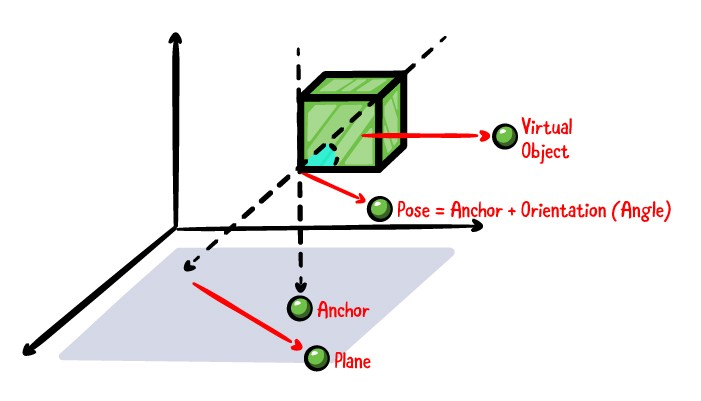
\includegraphics[width=0.8\textwidth]{./resources/images/UserInteraction/Anchor.jpeg}}%
			{Fonte: \url{https://medium.com/@jaaveeth.developer/arcore-81528569eb2c}}
			\caption{Oggetto virtuale in un piano}
			\label{fig: Oggetto virtuale in un piano}
		\end{figure}	

		\noindent 
		Nella modalità \emph{Plane Detection} la posa (posizione e orientamento) di un animale rimane invariata anche se l'ambiente circostante cambia. 
		\\
		La figura\vref{fig: rilevamento plane det} riporta degli esempi tratti dalla nostra applicazione in cui si può notare che il pinguino rimane nello stesso punto da qualsiasi prospettiva e distanza.
	
		\begin{figure}
			\centering
			\subfloat[][\emph{Pinguino da un'inquadratura vicina}]
			{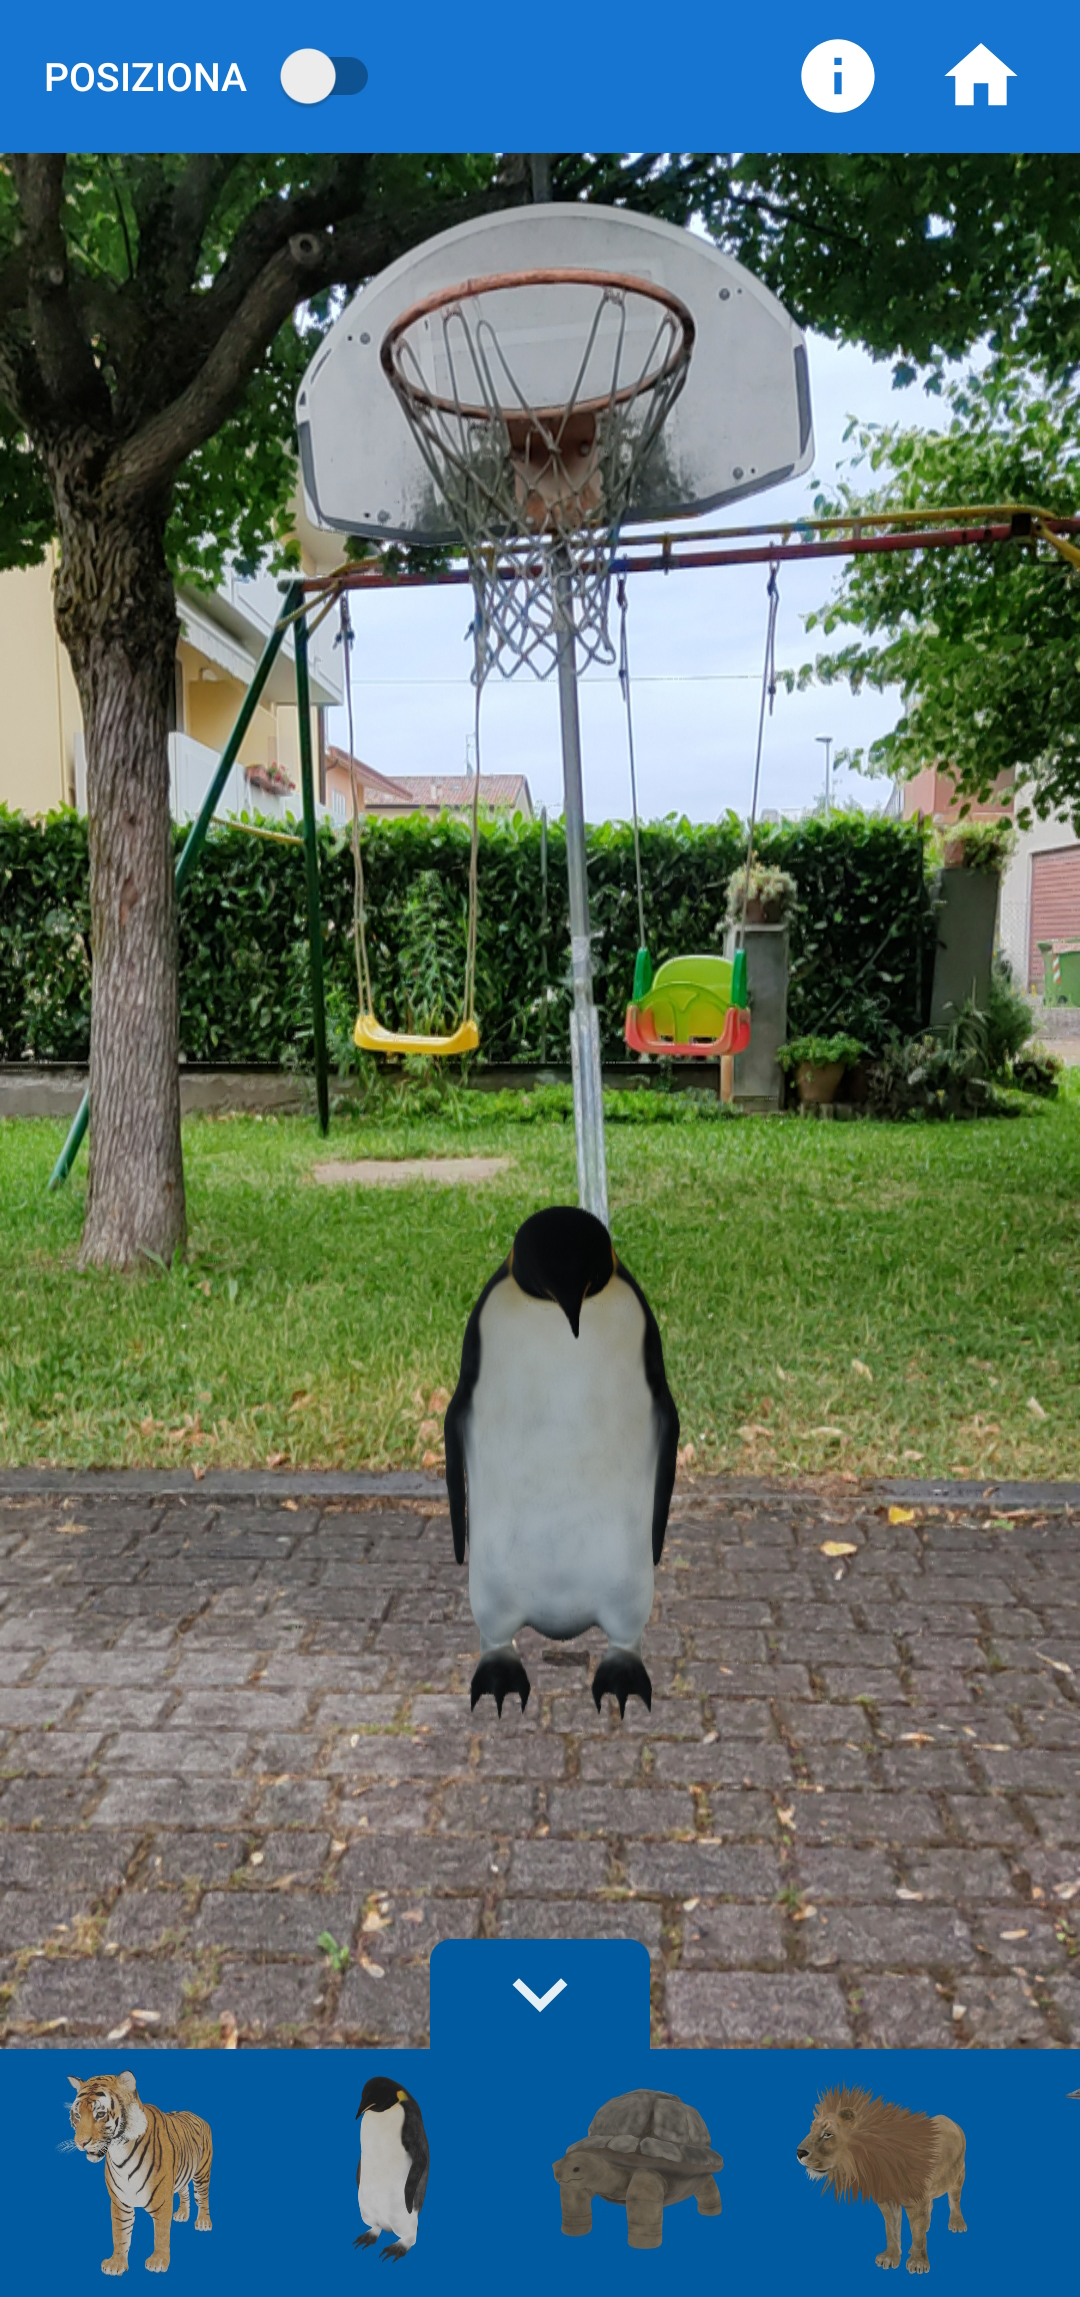
\includegraphics[width=0.28\textwidth]{./resources/images/AnchorTrackable/pingvicino.jpg}}  \quad
			\subfloat[][\emph{Pinguino da un'inquadratura lontana frontale}]
			{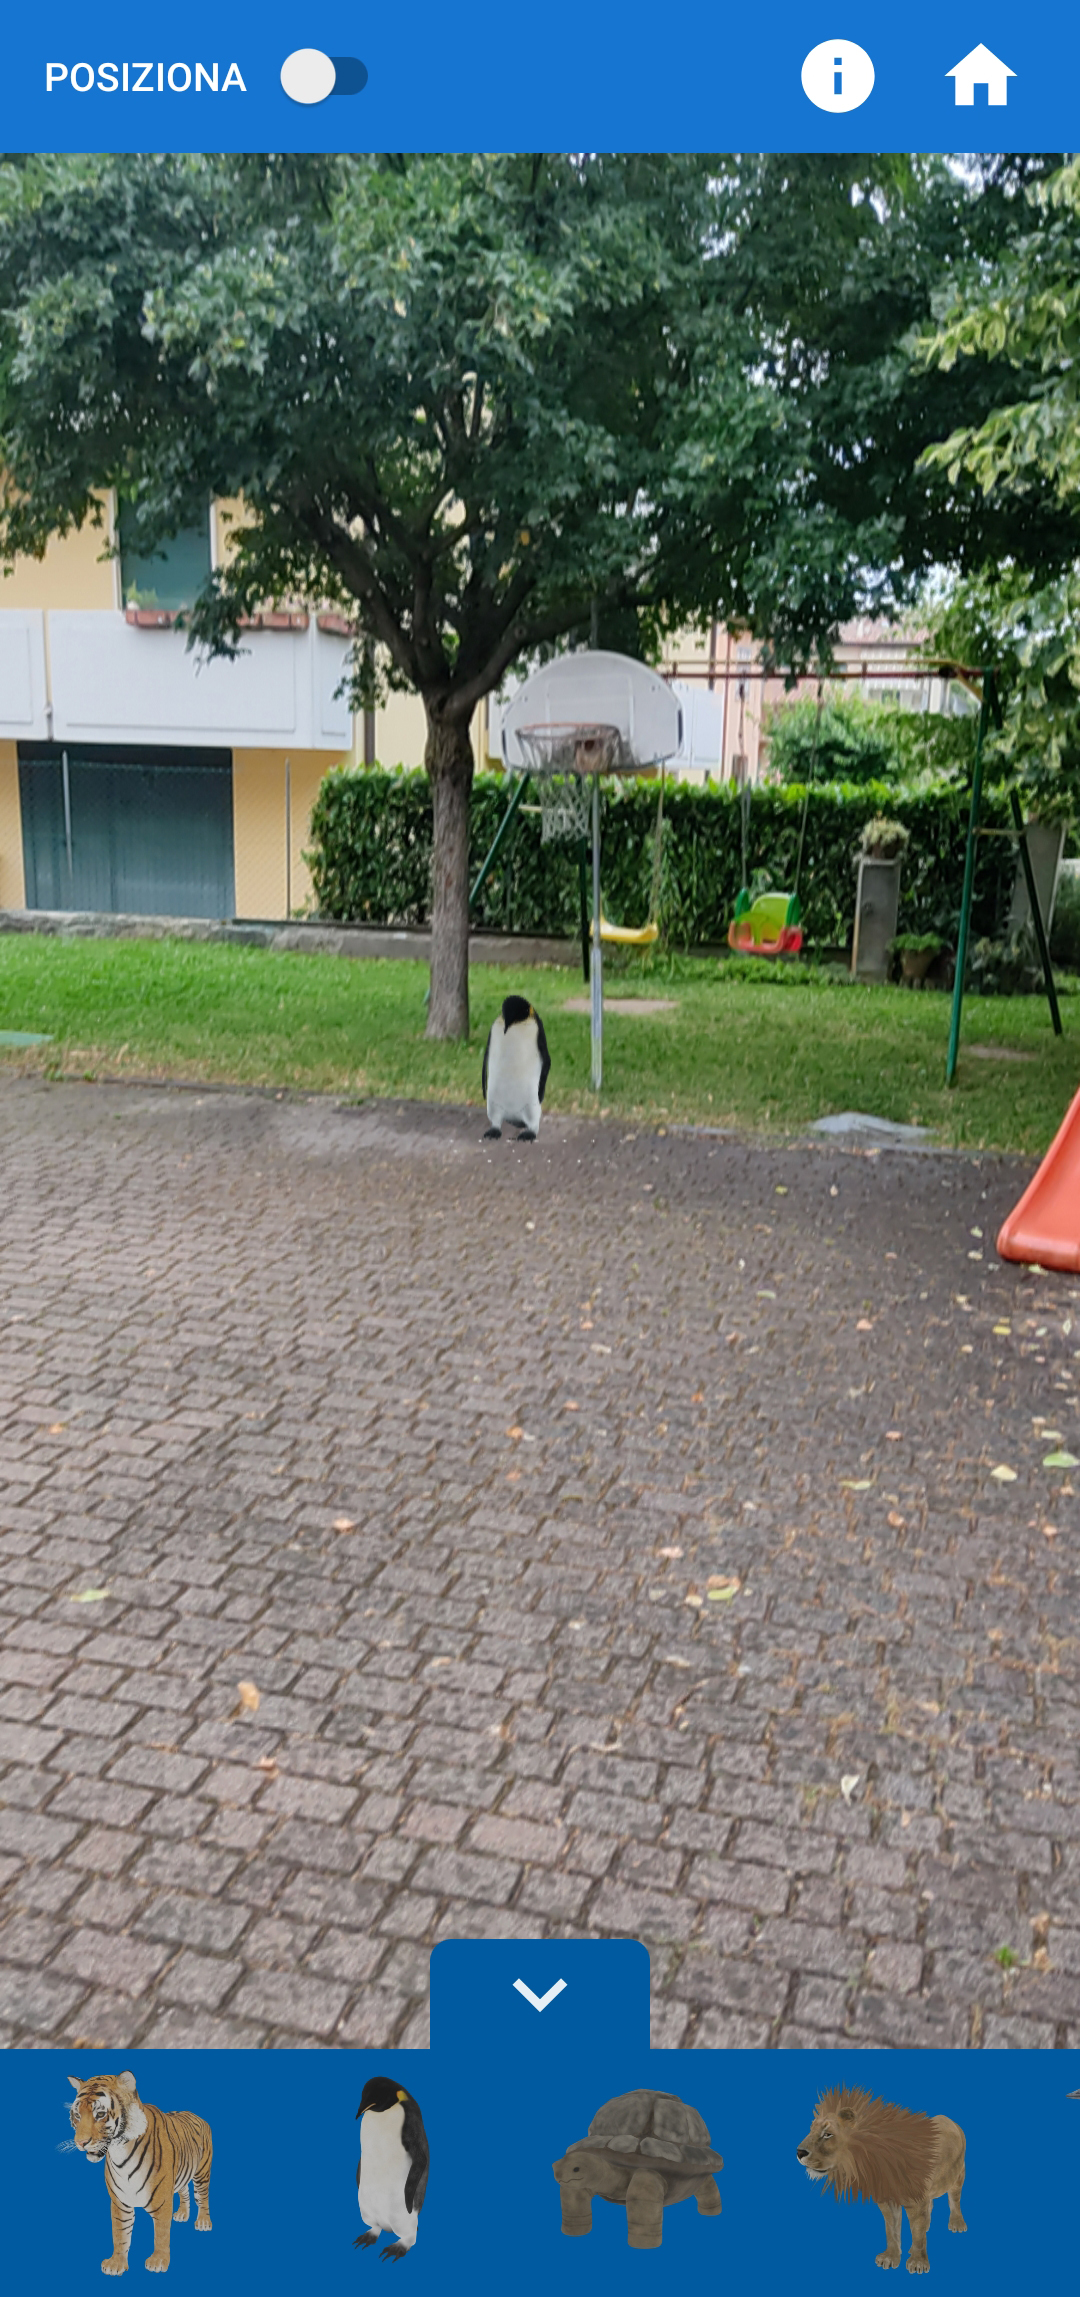
\includegraphics[width=0.28\textwidth]{./resources/images/AnchorTrackable/pinglontano1.jpg}} \quad
			\subfloat[][\emph{Pinguino da un'inquadratura lontana posteriore}]
			{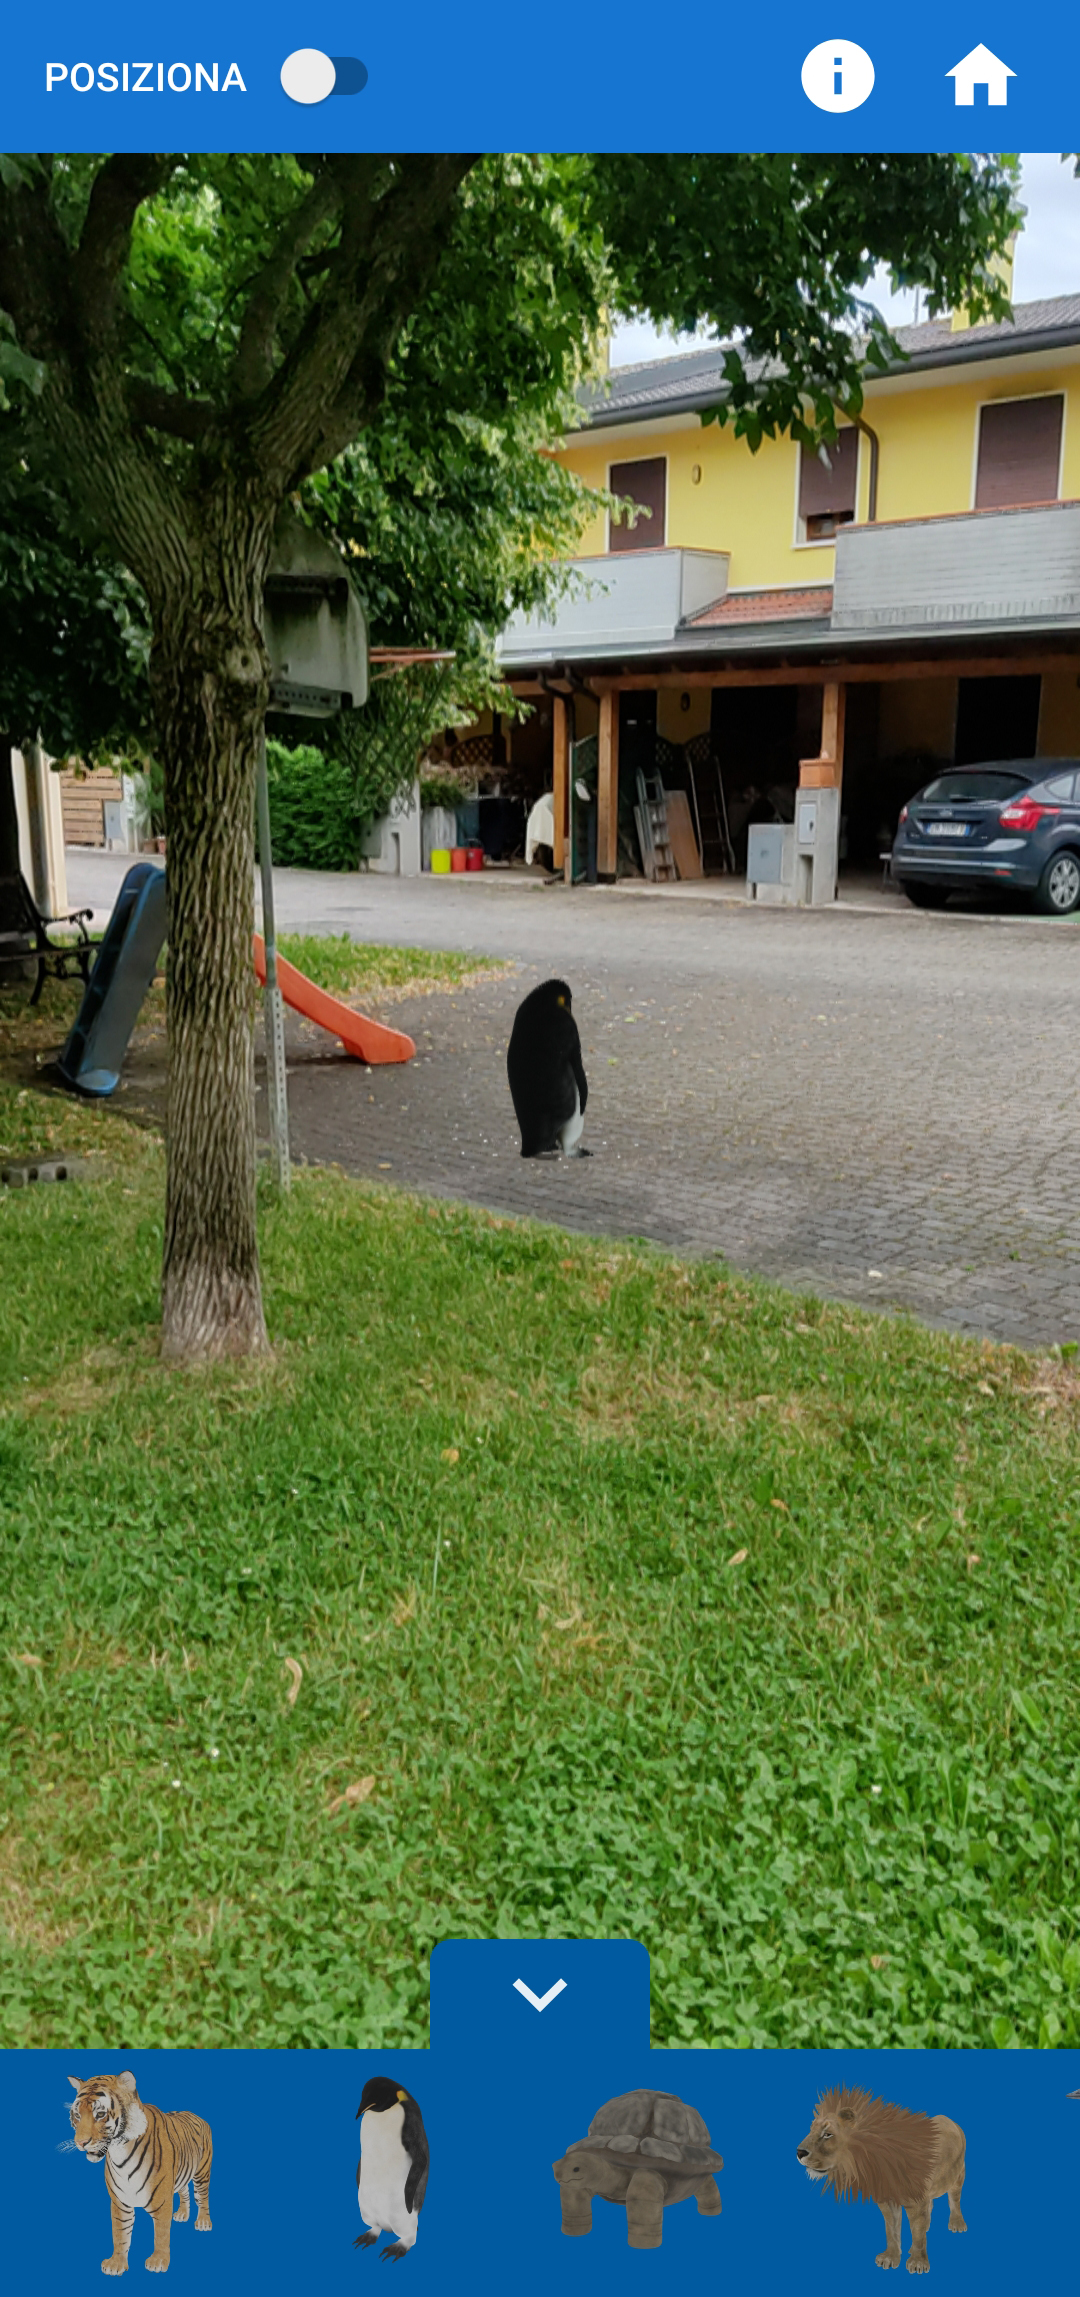
\includegraphics[width=0.28\textwidth]{./resources/images/AnchorTrackable/pinglontano2.jpg}}
			\caption{Esempio di inquadrature differenti in Plane Detection}
			\label{fig: rilevamento plane det}
		\end{figure}	
		
		\noindent
		La figura~\vref{fig: rilevamento augm img} tratta dalla nostra applicazione mostra che nella modalità \emph{Augmented Images} il pianeta rimane ancorato alla sua posizione.
	
		\begin{figure}
			\centering
				\subfloat[][\emph{Tracciamento immagine}]
				{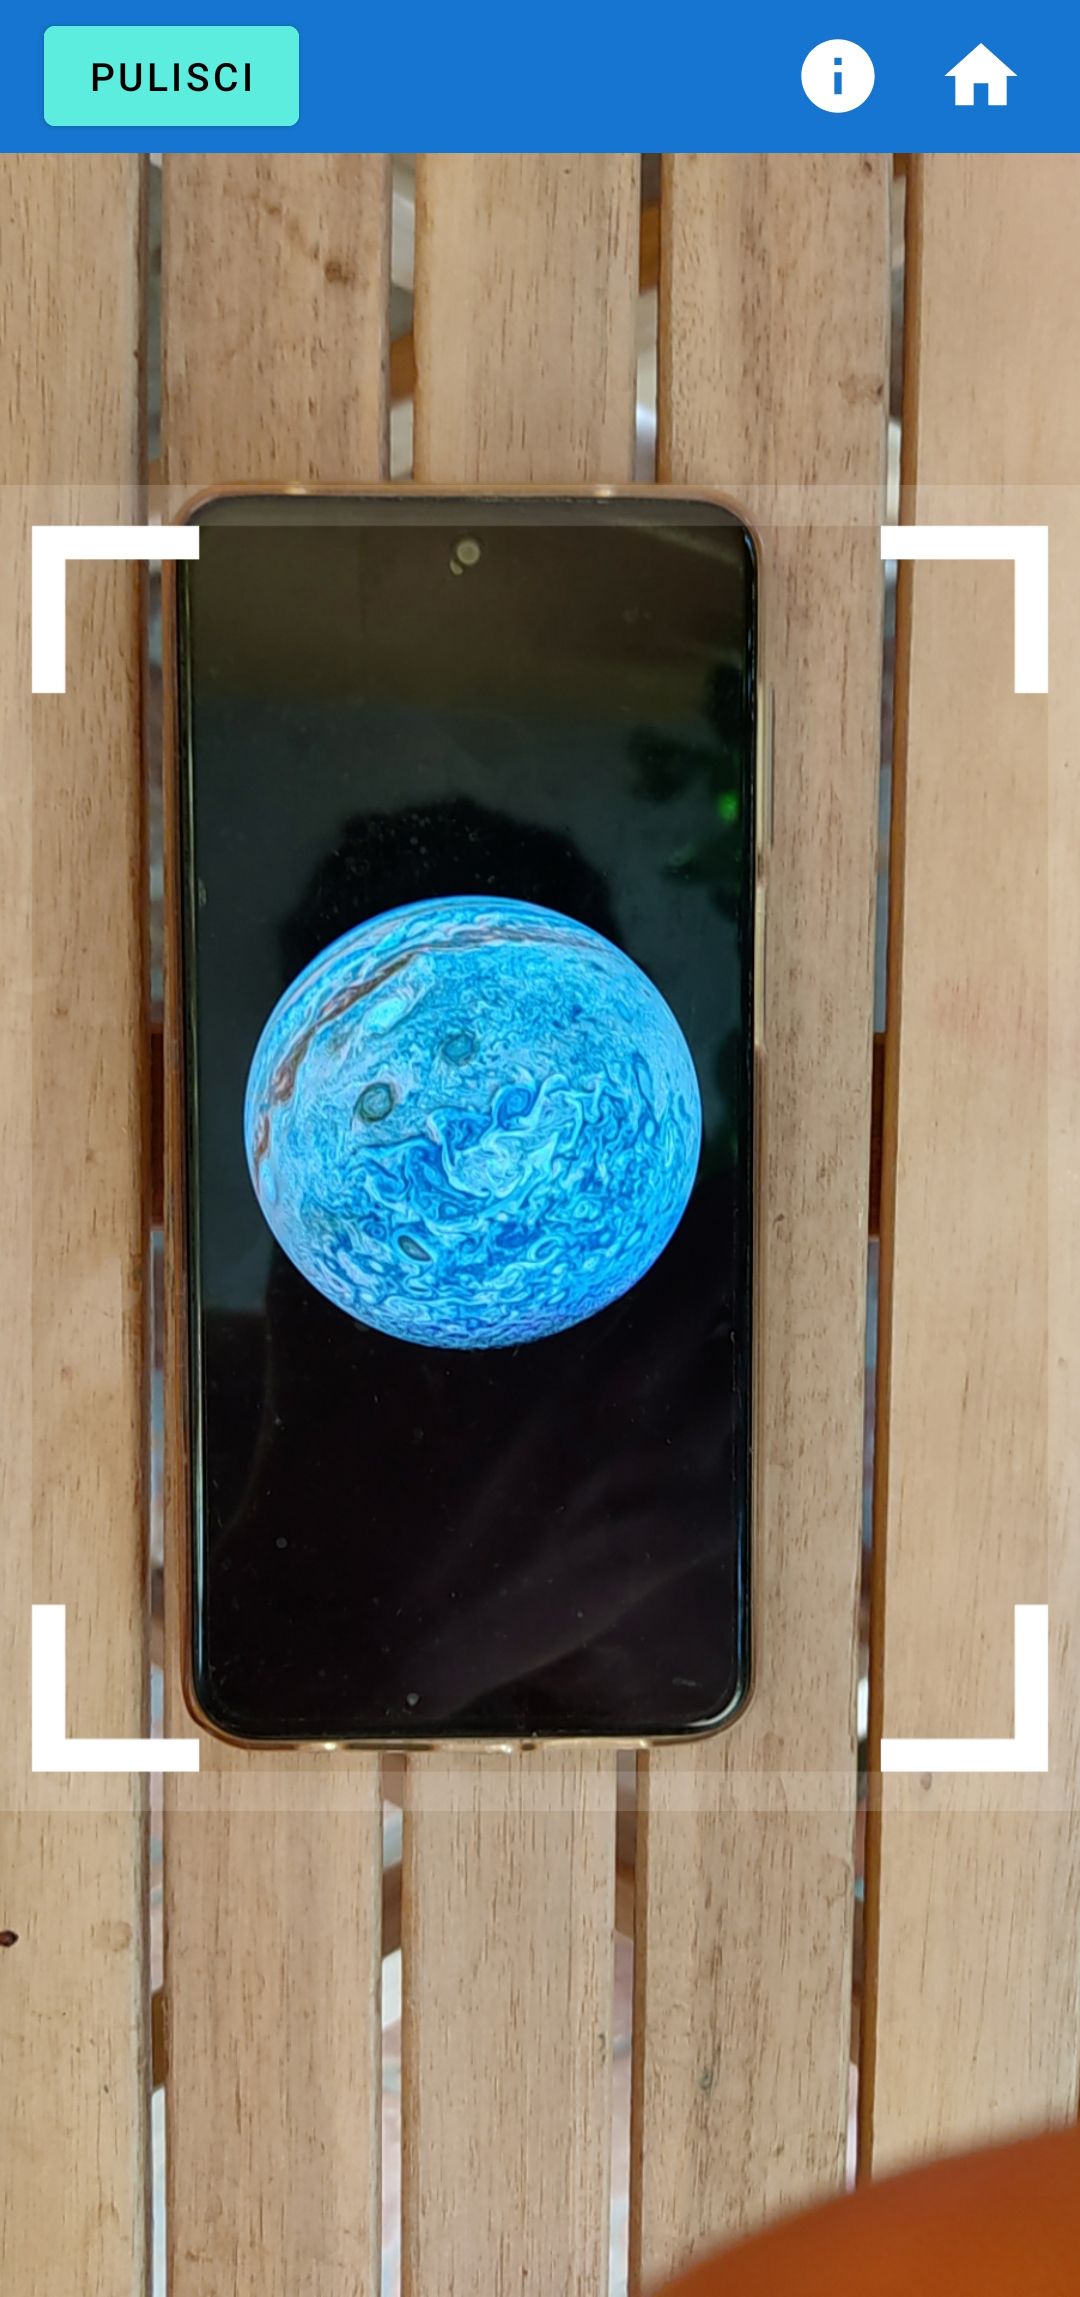
\includegraphics[width=0.28\textwidth]{./resources/images/AnchorTrackable/Giove2d.jpg}}  \quad
				\subfloat[][\emph{Giove da vicino}]
				{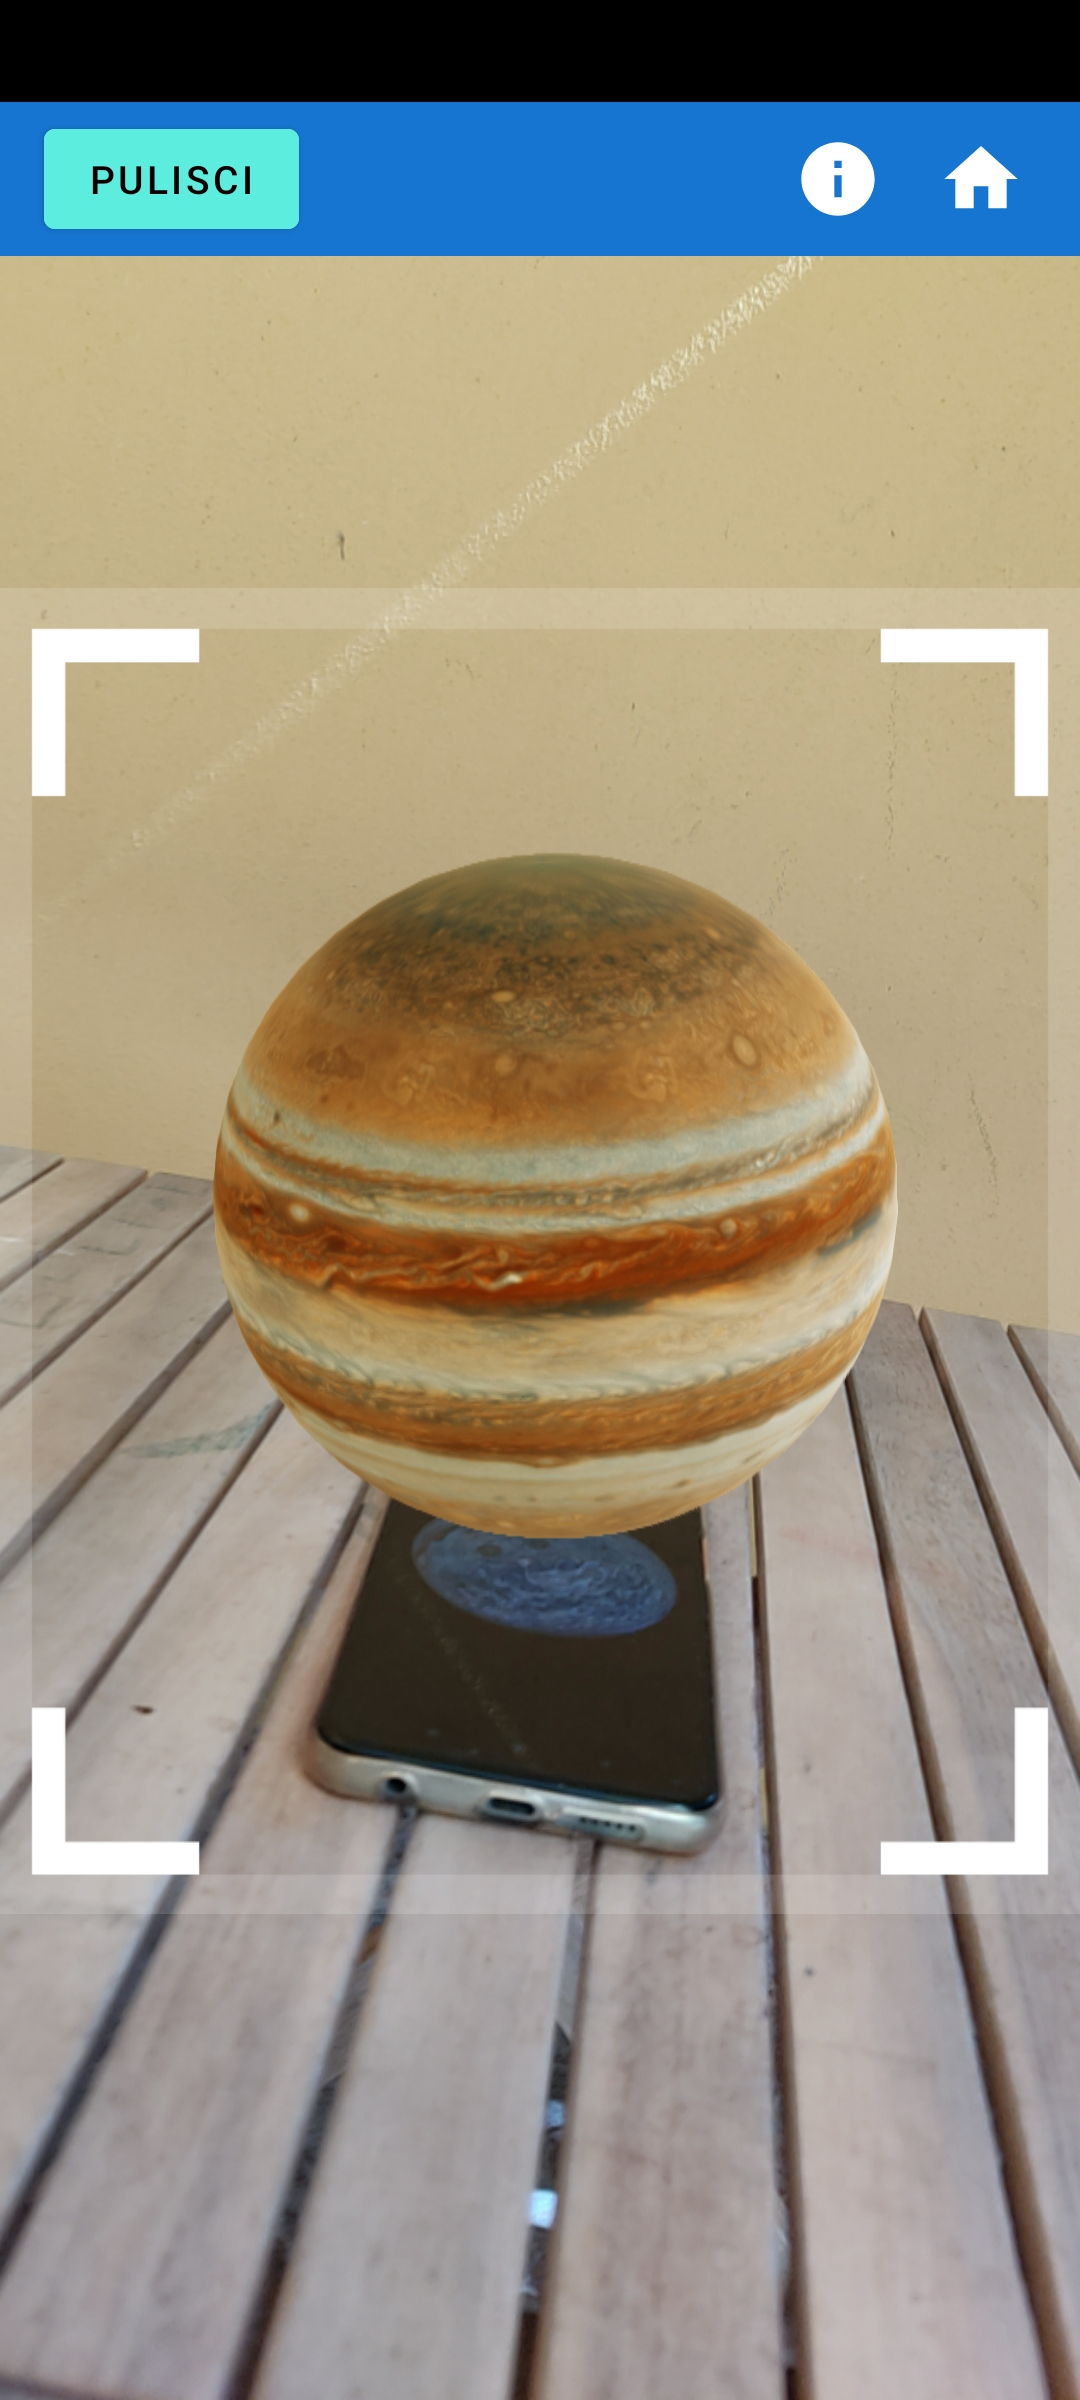
\includegraphics[width=0.28\textwidth]{./resources/images/AnchorTrackable/GioveVicino.jpg}} \quad
				\subfloat[][\emph{Giove da lontano}]
				{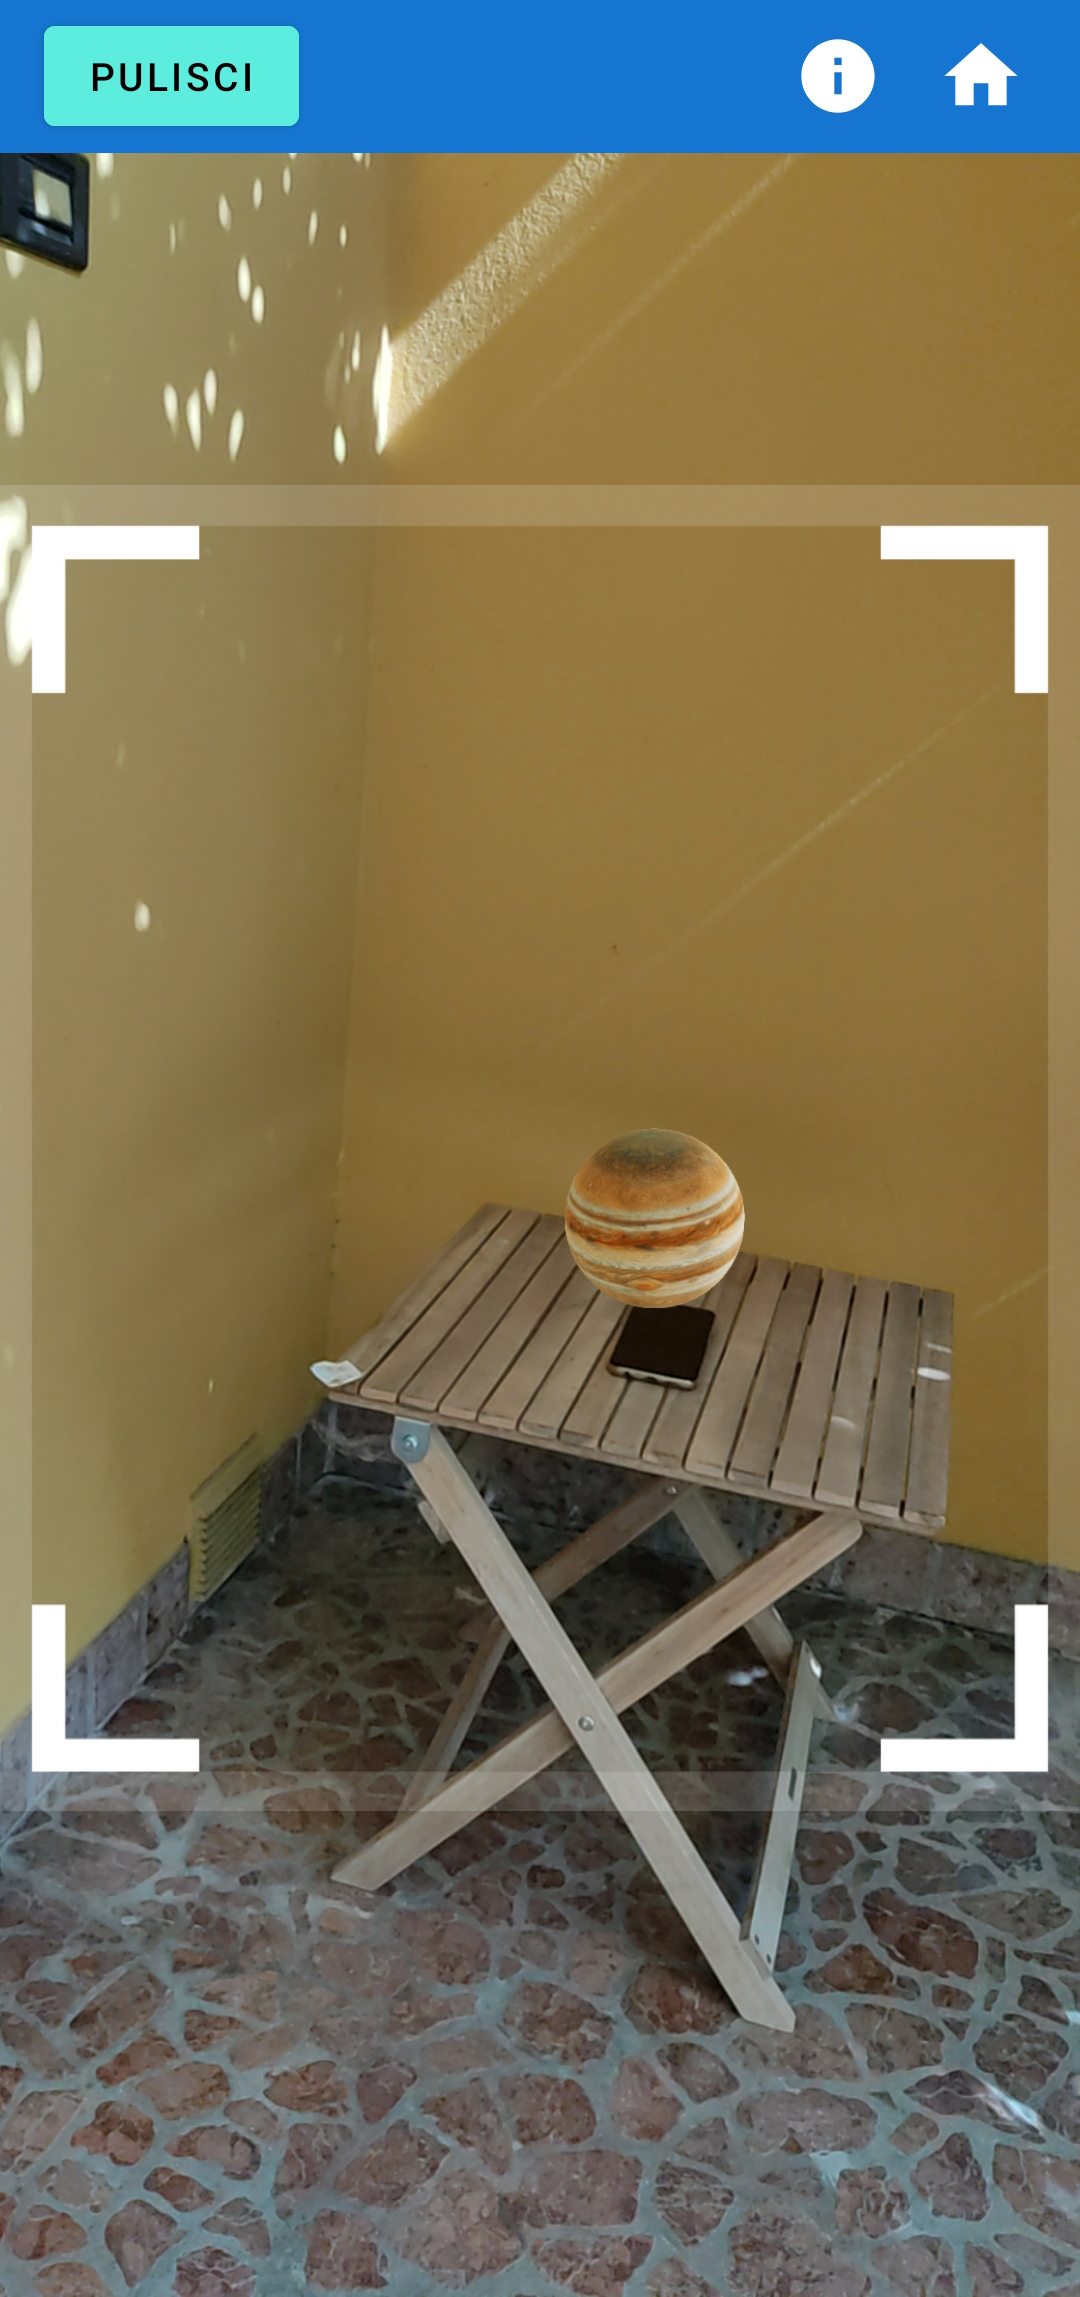
\includegraphics[width=0.28\textwidth]{./resources/images/AnchorTrackable/GioveLontano.jpg}}
			\caption{Esempio di rilevamento in Augmented Images}
			\label{fig: rilevamento augm img}
		\end{figure}
\end{document}